\documentclass{article}
\usepackage[final]{nips_2017}
\usepackage[utf8]{inputenc} % allow utf-8 input
\usepackage[T1]{fontenc}    % use 8-bit T1 fonts
\usepackage{hyperref}       % hyperlinks
\usepackage{url}            % simple URL typesetting
\usepackage{booktabs}       % professional-quality tables
\usepackage{amsfonts}       % blackboard math symbols
\usepackage{nicefrac}       % compact symbols for 1/2, etc.
\usepackage{microtype}      % microtypography
\usepackage{graphicx}
\usepackage{wrapfig}
\title{Family kinship Recognition Using Inception RestNet}

\author{
  Bruce Jianye Liu\\
  Department of Computer Science\\
  Stanford University\\
  \texttt{bruceliu@stanford.edu} \\
}


\begin{document}
% \nipsfinalcopy is no longer used

\begin{center}

\includegraphics[width=3cm, height=0.7cm]{CS230}
\end{center}

\maketitle

\begin{abstract}
Computer vision based face recognition experienced a significant progress over
last decade and most of face idenitification tasks focus on comparing two
face images to verify if they are the same person. However, Kinship
recoginition by face pictures is not quite popular in academia. As more
open family face dataset publicly accessible and new well-engineered deep
neural network architecture invented, state-of-art results on kinship
idenitificaiton becomes possible. In this paper, we trained a deep neural
network architecture based on a fine-tuned Inception ResNet v2 to identify
parent-child, siblings relationships by comparing two face pictures and
achieved 82\% accuracy on FIW test set, surpassing previous study about 7\%.
\end{abstract}

\section{Introduction}

Half of genetic information is shared between parents and children, and almost
the same amount of DNA are also shared among siblings in a family. People
biologically related often show some sort of delicate similiarities among each
other. This declicacy could be easily caught by human eyes, by observing faces
of their family photos. As computer vision performance improving during the
past decade, it becomes possible to use meachine learning to capture the
different. Computer vision based kinship recognition could lead variety of
usefull applications in real life such as missing-children parents matching,
family album organization, socal networking apps, lost sibling/relatives
searching, crime investigation.  In this paper, we propose a fine-tuned KinNet
model to identify the relationship between two faces -- parent-children,
sibling-sibling, none-kinship, and same person. We are able to achieve over 80
percent accuracy.

\section{Related Works}

Even thought many researcher have tried traditional approach to on image
recogintion tasks, Deep learning showed state-of-art achievement out-perform
other methods frequently in computer image tasks. One of well-known image
recognition tasks is ImageNet[5] classification, which contains 14 million
images labeled to roughly 22,000 catergories, and is widely used in literacy as
a large visual database for visual object recognition.

Starting from 2009, many neural network models are designed by researchers,
among them AlexNet[6] from University of Toronto in 2012, GoogLeNet
(Inception)[7] from Google in 2014, VGG[8] from Oxford Vision Geometry Group in
2015, and ResNet[9] form Microsoft Research showing significant impact on
academia. The error rate reached as low as 3.57\% surpassing human performance.

Beside Imagenet dataset, Labeled Faces in the Wild (LFW)[10] dataset and
Youtube Faces DB are widely used in face recognition tasks. Despite many other
non-deep learning models have good performance, deep neural network models keep
top records on this task, such as faceNet[2] designed by Schroff etc. achieved
99.63\% accuracy.

Similar to face verification problem, kinship recognition is another task that
attracts many researchers to put effect on.  [3] did some search on VGG-Face
net to classify family member,  decide whether a face belongs to a families,
and family kinship regcontion,determining whether two faces are
mother-daughter, monther-son, father-daughter, father-son, silbling relations.
They achieved about 75\% accuracy, surpassing human error rate.  While other
researchers focused on non-deep learning appraches such as hand-crafted
feature, face ecnodings, and metric learning, it is out of this paper's scope.

\section{Dataset}

\begin{wrapfigure}{l}{0.25\textwidth}
\caption{108x124 face sample}
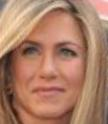
\includegraphics{img/P00241_face0}
\end{wrapfigure}

Families In The Wild (FIW) Database[1] is one of the largest and most
comprehensive database available for kinship recognition, published by Robinson
etc. in 2016. We use version 0.1.2 at writing time, which includes 13,188 faces
from 1018 families. Event though it has 11 kinship types, father-daughter
(F-D), father-son (F-S), mother-daughter (M-D), mother-son (M-S),
brother-brother (B-B), sister-sister (S-S), grandfather-granddaughter (GF-GD),
grandfather-grandson (GF-GS), grandmother-granddaughter (GM-GD),
grandmother-grandson (GM-GS). Siblings and parent-child types are what most
relavent to our research. By adding up 64,669 F-D, 46,143 F-S, 68,935 M-D, 48,
and 940 M-S types, we get 22,687 parent-child photos and for sibling types it
contains 55,937 pair of photos. All face images are cropped from public family
photos with idential size 108*124*3 and manually labeled. For the same person
faces, we generated them by selecting pictures with the same FaceID. Similarly
non-related picture pairs are created by combining one image in unrealted
folder under the family ID folder and one of the faces in the family.

\begin{table}[h]
	\centering
	\begin{tabular}{ | c || r r | }
		\hline
		\multicolumn{3}{|c|}{face-pair image distribution} \\
		\hline
		pair types&face-pair number&percentage\\
		\hline
			parent-child & 228,687 &21.17\% \\
			siblings & 55,937 & 5.18\% \\
			same & 230,938 & 21.38\% \\
			unrelated & 564,496 & 52.27\% \\
		\hline
			& 1,080,058 & \\
		\hline
	\end{tabular}
	\caption{Training data distribution}
	\label{table:1}
\end{table}

Table 1 shows all the data distribution that we have. We managed to assemble
nearly 1 million image pairs from FIW dataset by scanning folders, permutation
image pairs, and summing up existing face pairs. The amount of family faces and
unrelated images pairs is over 500,000 nearly 52\% of all data. Parent-child
and the same face pairs contain almost the equal number of images, about
230,000 respectly, nearly 21\%.  On the other hand, only 5\% of data are
sibling face pairs, which may affect our model on predicting sibling kinship.
In practice, we forsake some data in order to make our dataset eveno on each
catergory.

\section{Methods and Models}

FaceNet has been proved in paper [2] that it performances very well in face
recognition tasks. We borrowed some idea from FaceNet architecture by tweaking
the existing model to classify kinship face image pairs.

\begin{figure}[h]
	\caption{Our modified model}
	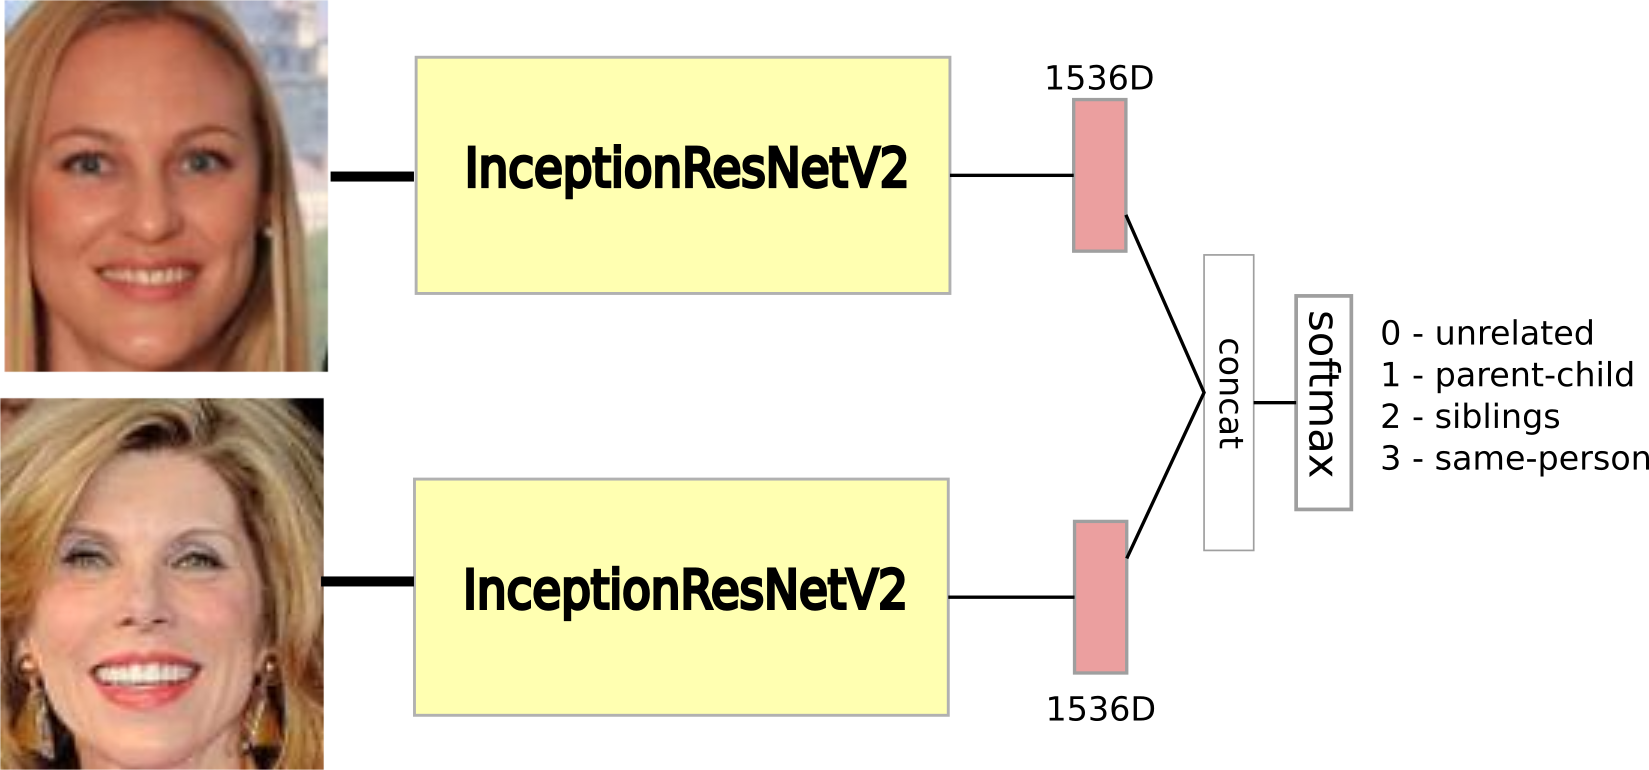
\includegraphics[width=1\textwidth]{img/model_pic1}
	\centering
\end{figure}

The last facenet implementation is based on InceptionResNetv2[11], which
possibly have a better performance than VGG-Face net. However it is very
expensive to train weights from scratch as it contains over 1 million
parameters. So instead of starting from randomized weights, we took a model
with a pre-train weights on ImageNet. This transfer-learning approach could
reduce our training time.

To handle the uneven training dataset, we take 50,000 images from each
catergory, and shuffle the whole 200K images, split 6000 images pair sample as
a test set, leaving the rest of the data as training. At each epoch we randomly
extract 10,000 training images from training set with batch sizes 16, in order
to fit our memory.  Even thought we forsake some data volunterily, it is
enought to train the model. We trained two models with this training dataset
arrangement.

In the first model, I took the InceptionResNetV2 model, removing the last full
connection layer and add global average last layer with 1536 dimension output,
following two dense layer with 1024, 128 units seperately. The finally layer is
a 4 node softmax output. For each face pair, I feed them into InceptionResNet
and get two 1536 vector which are concatenated into 3072 vector. This will feed
into dense layers to produce 4 output. Table 2 show detail architecture.

\begin{table}[h]
	\centering
	\begin{tabular}{ | l | c | c | c | c |}
		\hline
		\textbf{layers}&\textbf{size-in}&\textbf{size-out}&\textbf{param}&\textbf{FLPS}\\
		\hline
			Input1 & 299x299x3 & & 0 & \\
			Input2 & 299x299x3 & & 0 & \\
			InceptionResNetV2 & 299x299x3 & 1x1536 & 75M & 75M \\
			InceptionResNetV2 & 299x299x3 & 1x1536 & 75M & 75M \\
			concat & 2x1536 & 1x3072 & & 0 \\
			fc1 & 1x3072 & 1x1024 & 3M & 3M \\
			fc2 & 1x1024 & 1x128 & 131K & 131K \\
			softmax & 1x1024 & 1x4 & 4100 & 4100 \\
		\hline
	\end{tabular}
	\caption{KinNet Layers Model I}
	\label{table:2}
\end{table}

After serveral epochs of training, It started to converge, the best result we
get with 0.677 accuracy, with 1.580017 lost. It trained continuely over a
serveral days. Due to computer memory limitation, it is impossible to fit all
training image. We choose to split train set to 5000 images for each training
session, in over 5 session. It starts to overfit, training accuracy up to 98\%
but test set about 68\%.

To handle over fitting problem with model I, we created Model II (table 2) by
removing these two middle full-connected layers and keeping only the last
softmax layer of four units. This modification works pretty well during
training sessions.  We didn't reuse the trained weights on model I, instead the
model II were trained on ImageNet weights Its accuracy and loss changed
grandually. We chose 0.01 learning rate with Adam Opitimization on the first 8
epchos, until its test accuray reaced 65\%. Themodel started over shooting
while training accuracy bumped above 80\%.  We reduced learning rate to 0.001
for next 5 epochs, and its test accuracy slowly climbed over 75\%. Learning
rate 0.0001 was used in the last training session to further boost test
accuracy to 82\%. After 82\% its performance won't improve even if we adjust
learning rate.

\begin{table}[h]
	\centering
	\begin{tabular}{ | l | c | c | c | c |}
		\hline
		\textbf{layers}&\textbf{size-in}&\textbf{size-out}&\textbf{param}&\textbf{FLPS}\\
		\hline
			Input1 & 299x299x3 & & 0 & \\
			Input2 & 299x299x3 & & 0 & \\
			InceptionResNetV2 & 299x299x3 & 1x1536 & 75M & 75M \\
			InceptionResNetV2 & 299x299x3 & 1x1536 & 75M & 75M \\
			concat & 2x1536 & 1x3072 & & 0 \\
			softmax & 1x1024 & 1x4 & 4100 & 4100 \\
		\hline
	\end{tabular}
	\caption{KinNet Layers Model II}
	\label{table:3}
\end{table}


\begin{figure}[h]
	\caption{Test and Training Accuracy}
	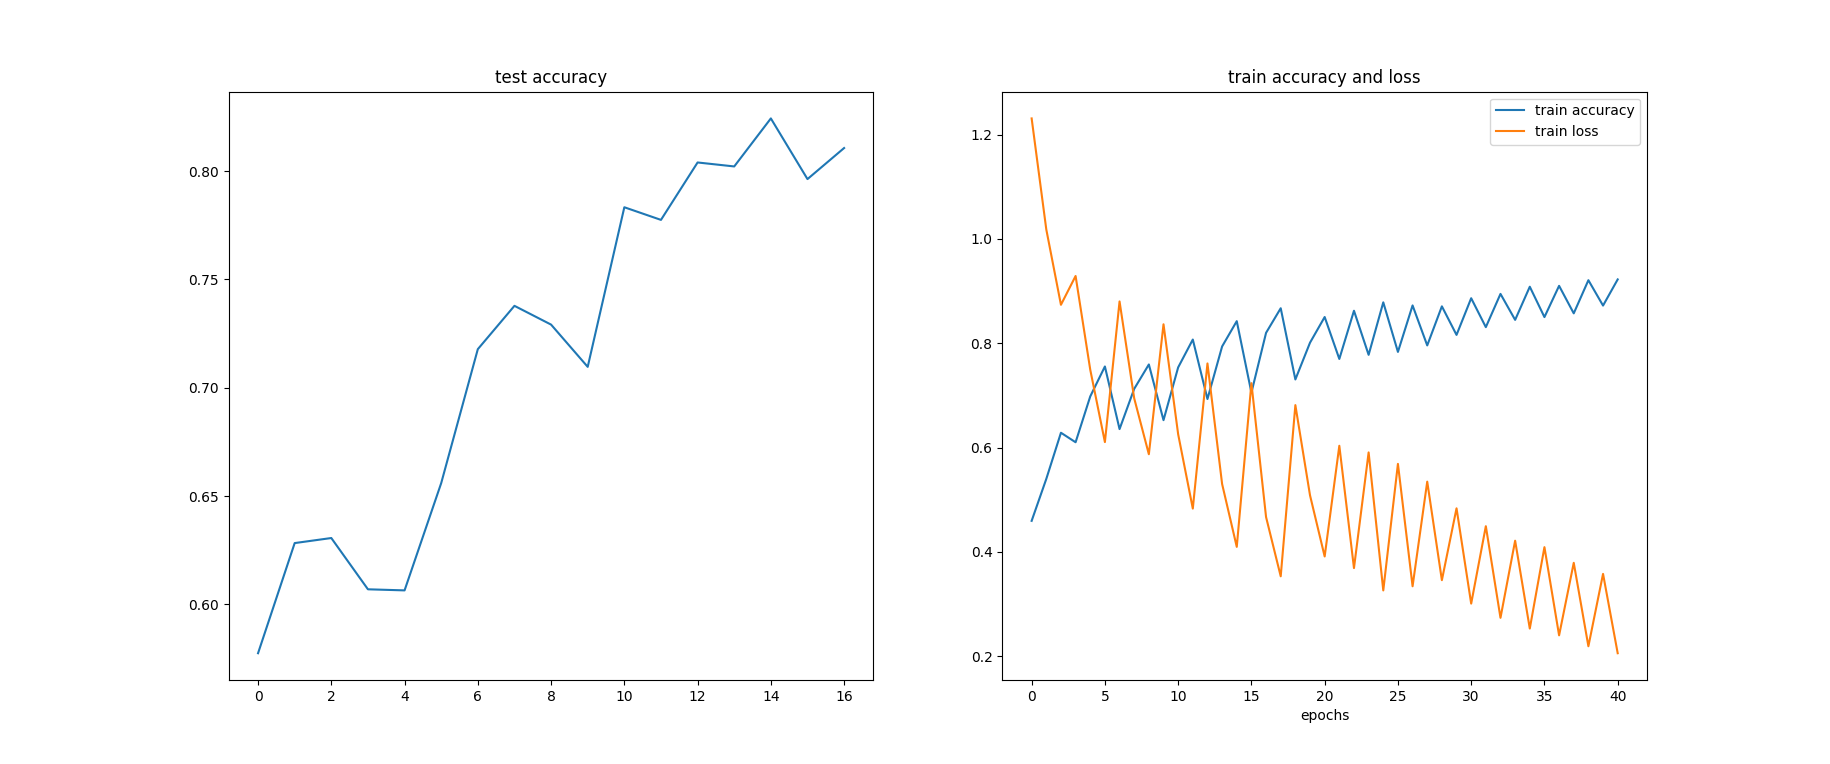
\includegraphics[width=1\textwidth]{img/loss_accuracy}
	\centering
\end{figure}

\section{Conclusion/Future Work }
Summarize your report and reiterate key points. Which algorithms were the highestperforming?
Why do you think that some algorithms worked better than others? For
future work, if you had more time, more team members, or more computational resources,
what would you explore?

By iterative adjusting hyperparmeters of Model II, we attained 82\% test
accuracy on FIW dataset, though the first model didn't get ideal result. It is
proved that the InceptionResNet performed well not only on basic object
recognition task but also on face recognition tasks. Further modification on
our model could be also worthy to try in future experiment, such as computing
consin similarity of two face images encoding, using k-neigbhour algorithm to
cluster the encoding, or changing some layers of InceptionResNet.

Even though approximate half of genes are shared among family members, solely
relying on face pairs for kinship verification might be hard to achieve higher
accuracy. If people without any family relation look simliar to each other,
even human might misjudge their relationship. Beside face likeness, gene
simliarity shared among siblings, generations could also exhibit in term of
height, skin color, nail shape, toes length, ear contours, hand size etc. These
information couldn't present in face images. Adding these additional
information in to our model, it could boost our model significantly. Due to
time limitation and team size, we aren't able to collect this data.

github repository: https://github.com/brucelau-github/cs230

\newpage
\section*{References}
\medskip
\small
[1] Robinson, Joseph P., et al. Families in the Wild (FIW): Large-Scale Kinship
Image Database and Benchmarks. {\it Proceedings of the 2016 ACM on Multimedia
Conference} - MM '16, 2016, doi:10.1145/2964284.2967219.

[2] Schroff, F., Kalenichenko, D., \& Philbin, J. (2015). FaceNet: A unified
embedding for face recognition and clustering. {\it 2015 IEEE Conference on
Computer Vision and Pattern Recognition (CVPR)}. doi: 10.1109/cvpr.2015.7298682

[3] Wang, S., Robinson, J. P., \& Fu, Y. (2017, May). Kinship verification on
families in the wild with marginalized denoising metric learning. {\it In 2017 12th
IEEE International Conference on Automatic Face \& Gesture Recognition (FG 2017)
(pp. 216-221). IEEE}.

[4] Szegedy, C., Ioffe, S., Vanhoucke, V., \& Alemi, A. A. (2017, February).
Inception-v4, inception-resnet and the impact of residual connections on
learning. In {\it Thirty-first AAAI conference on artificial intelligence}.

[5] Deng, J., Dong, W., Socher, R., Li, L.-J., Li, K.,\& Fei-Fei, L. (2009).
ImageNet: A large-scale hierarchical image database. In {\it 2009 IEEE
conference on computer vision and pattern recognition} (pp. 248-255).

[6] Krizhevsky, Alex., Sutskever, I., \& Hinton, G. E. (2012). Imagenet
classification with deep convolutional neural networks. In {\it Advances in
neural information processing system} (pp. 1097-1105).

[7] Szegedy, c., Liu, W., Jia, Y., Sermanet, P., Reed, S., Anguelov, D., ... \& Rabinovich, A. (2015). Going deeper with convolutions. In {\it Proceedings of the IEEE conference on computer vision and pattern recognition} (pp. 1-9)

[8] Simonyan, K., \& Zisserman, A. (2014). Very deep convolutional networks for large-scale image reognition. {\it arXiv preprint arXiv}: 1409. 1556.

[9] He, K., Zhang, X., Ren, S., \& Sun, J. (2016). Deep residual learning for image recognition. In {\it Proceedings of the IEEE conference on computer vision and pateern recognition} (pp. 770-778).

[10] Huang, G. B., Ramesh, M., Berg T., \& Learned-Miller, E. (2007) Labeled faces in the wild: a database for studying face recognition in unconstraned environments. In {\it Technical Report} 07-49, October 2017

[11] Szegedy, C., Ioffe, S., Vanhoucke, V., \& Alemi, A. A. (2017, February). Inception-v4, inception-resnet and the impact of residual connections on learning. In {\it Thirty-first AAAI conference on artificial intelligence}.

\end{document}
